% Titre de la premiere partie
\section{Le problème}

\begin{frame}
\frametitle{Sommaire}
    \tableofcontents[currentsection]
\end{frame}

%%%%%%%%%%%%%%%%%%%%%%%%%%%%%%%%%%%%%%%%%%%%%%%%
% Première diapo
%%%%%%%%%%%%%%%%%%%%%%%%%%%%%%%%%%%%%%%%%%%%%%%%
\begin{frame}
\frametitle{Introduction au problème}
\framesubtitle{Micromouse}

\begin{itemize}
	\item Course de robots appelées "souris" dans un labyrinthe :

    \begin{figure}
        \def\stackalignment{r}
        \stackunder{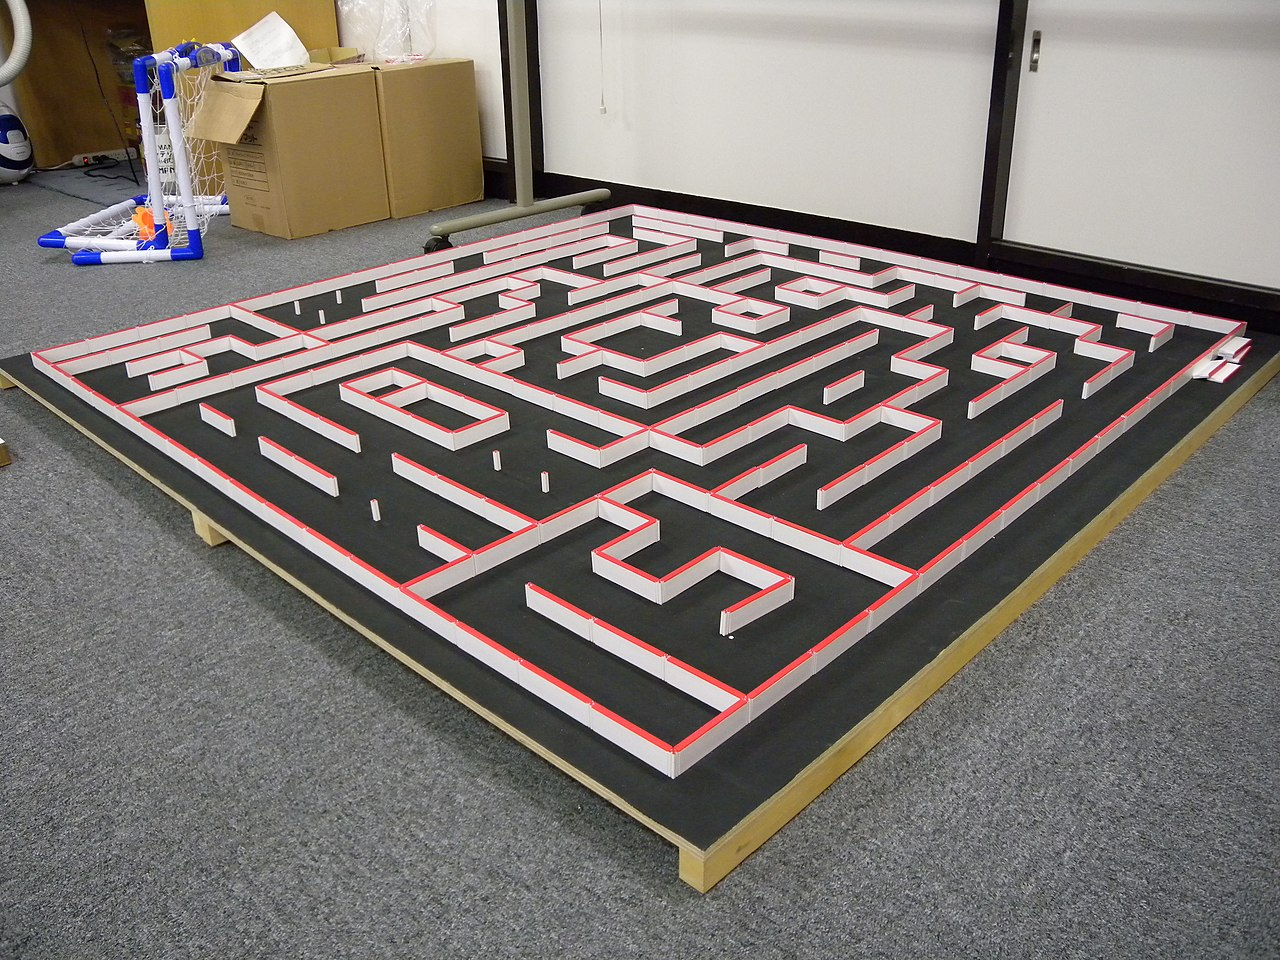
\includegraphics[width=0.4\linewidth]{assets/Micromouse_maze.jpg}}%
           {\sources
            Source: Osamu Iwasaki}
    \hfill
        \def\stackalignment{r}
        \stackunder{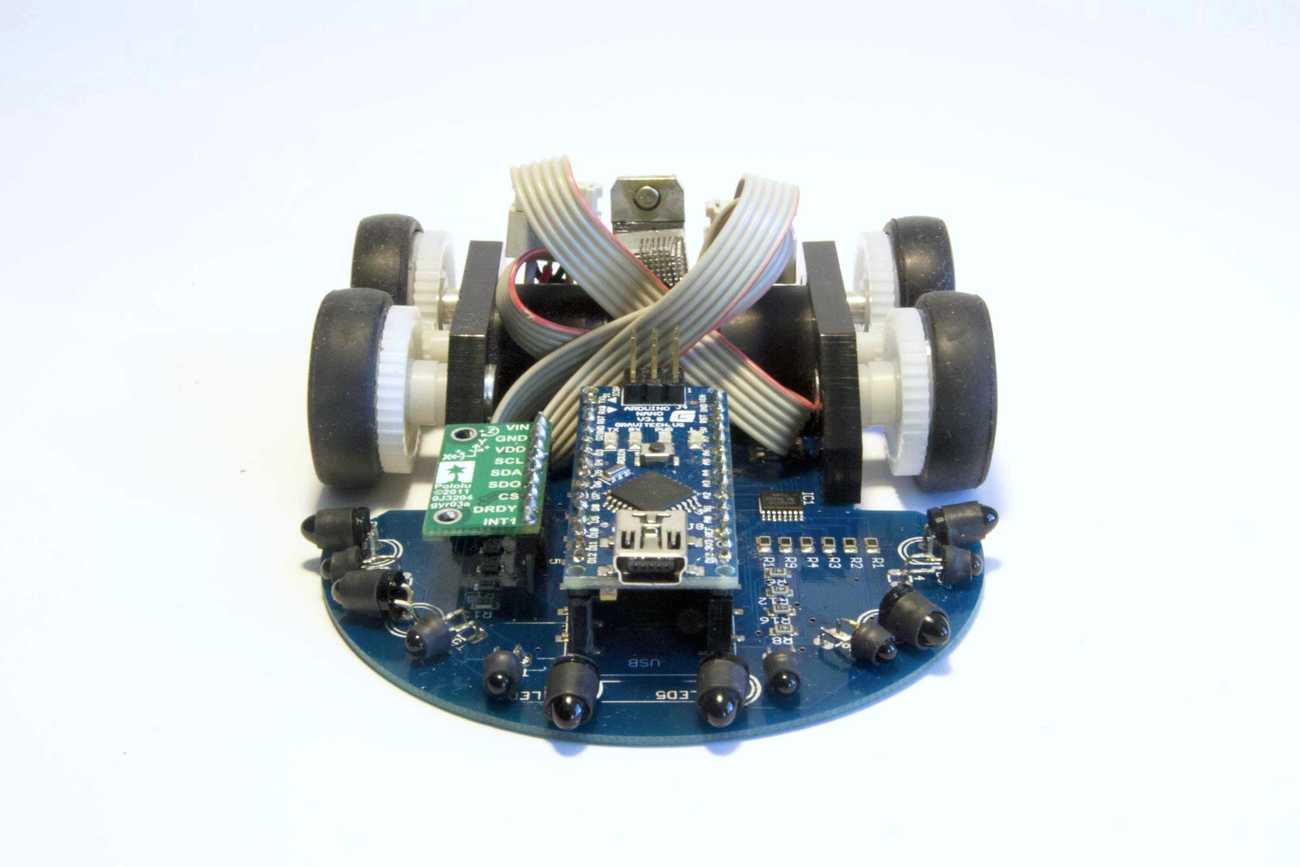
\includegraphics[width=0.4\linewidth]{assets/mouse-3.jpg}}%
           {\sources
            Source: \url{alexhadik.com/work/micromouse/}}
	\end{figure}
	\item	<2-> Les règles ? Quelques minutes pour :
    \begin{enumerate}
        \item Explorer le labyrinthe, enregistrer la position des murs
        \item Calculer le chemin le plus rapide
        \item Faire plusieurs tentatives de courses
    \end{enumerate}
\end{itemize}

\end{frame}

%%%%%%%%%%%%%%%%%%%%%%%%%%%%%%%%%%%%%%%%%%%%%%%%
% Deuxième diapo
%%%%%%%%%%%%%%%%%%%%%%%%%%%%%%%%%%%%%%%%%%%%%%%%
\begin{frame}{Position du problème}
    \begin{itemize}
        \item \textbf{Objectif 1:} Trouver le chemin le plus rapide
        \item<2-> \textbf{Objectif 2:} Éviter les collisions avec les obstacles
        \item<3-> \textbf{Objectif 3:} Temps de calcul le plus court possible
    \end{itemize}
    \begin{figure}
        \visible<4->{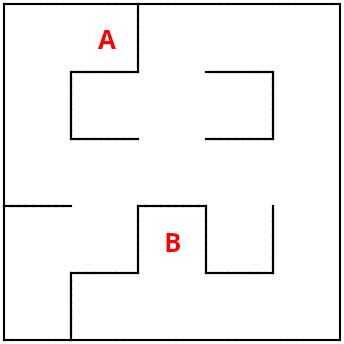
\includegraphics[width=0.35\linewidth]{assets/empty_5x5.png}}
        \visible<4->{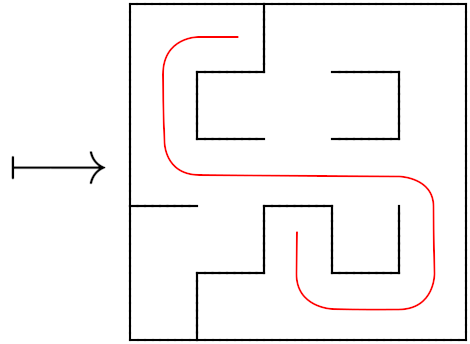
\includegraphics[width=0.48\linewidth]{assets/path_5x5.png}}
    \end{figure}
\end{frame}